\documentclass{article}

\usepackage[letterpaper]{geometry}
\usepackage{amsmath}
\usepackage{amssymb}
\usepackage{siunitx}
\usepackage{graphicx}
\usepackage{tikz}
\usetikzlibrary{shapes.geometric}

\title{4261 HW 6}
\author{Duncan Wilkie}
\date{?}

\begin{document}

\maketitle

\section*{1a}
We have an effective Schr\"odinger equation, following the cited problem,
\[
  E\phi_{n}=\epsilon\phi_{n}-t(\phi_{n+1}+\phi_{n-1})
\]
Applying the ansatz $\phi_{n}=e^{ikna}/\sqrt{N}$, where $N$ is some normalization constant, we get
\[
  Ee^{ikna}=\epsilon e^{ikna}-te^{ik(n+1)a}-te^{ik(n-1)a}
  \Leftrightarrow E=\epsilon-t(e^{ika}+e^{-ika})
  =\epsilon-2t\cos(ka)
\]
A plot with random values for the constants appears below.
\[
  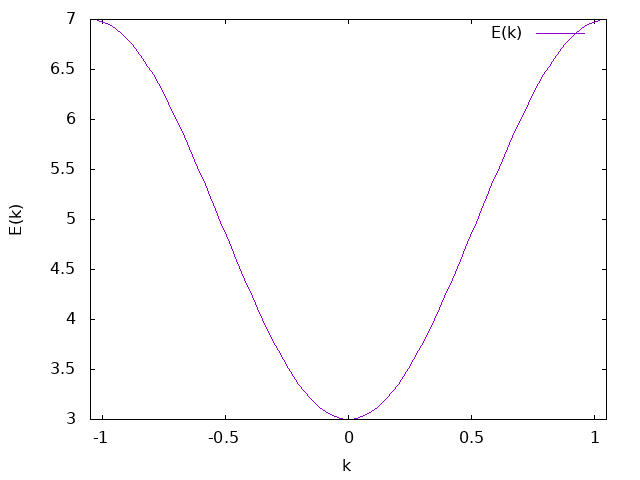
\includegraphics[scale=.8]{plot1.png}
\]
If there are $N$ sites, and we have periodic boundary conditions $k=k+2\pi/a$, the total system $k$ is quantized as $k=2\pi m/(Na)$,
i.e. there are $N$ values of $k$ corresponding bijectively to $N$ eigenstates of the system.
Approximating $\cos x= 1-x^{2}/2$ near zero,
\[E(k)\approx \epsilon-2t+tk^{2}a^{2}\]
Comparing this to the free electron dispersion,
\[
  \frac{\hbar^{2} k^{2}}{2m^{*}}=ta^{2}k^{2}
  \Leftrightarrow m^{*}=\frac{\hbar^{2}}{2ta^{2}}
\]
The density of states is by definition
\[
  g(E)=\frac{dN}{dE}=\frac{dN}{dk}\frac{dk}{dE}
\]
The first term is constant, since the number of states per unit $k$ is constant; it is equal to $Na/2\pi$.
The second is, from the dispersion relation, $1/2ta\sin(ka)$, so in total we have
\[
  g(E)=\frac{N}{4\pi t\sin(ka)}
\]
Monovalent atoms imply half-filled bands, in which case the Fermi surface (the boundary between filled and unfilled states) occurs halfway
through the first Brillouin zone at $k=\pi/2a$ and $k=-\pi/2a$, which corresponds to a density of states $N/4\pi t$.
Heat capacity in terms of the density of states is, following section 4.2,
\[
  C_{V}=\tilde{\gamma}k_{B}^{2}g(E_{F})TV
  =\tilde{\gamma}k_{B}^{2}NTV/4\pi t
\]
If the atoms are divalent, then the band is fully filled, which means there's no way the energy of the system can change as the temperature
changes, i.e. $C_{V}=0$.
Similarly, the spin susceptibility is also zero, since there are no available states for the electrons to move into and align with the
applied magnetic field, i.e. $M(H)=0$.

\section*{1b}
Our unit cell is now expanded to include two adjacent atoms, so we have a system of effective Schr\"odinger equations of the same
type as above:
\[
  E\phi_{n,A}=\epsilon_{A} \phi_{n,A}-t(\phi_{n,B}+\phi_{n-1,B})
\]
\[
  E\phi_{n,B}=\epsilon_{B}\phi_{n,B}-t(\phi_{n+1,A}+\phi_{n,A})
\]
where $\phi_{n,A}$ ($\phi_{n,B}$) denotes the contribution to the $n$th site wave function from atom $A$ ($B$).
Using ans\"atze
\[
  \phi_{n,A}=Ae^{ikna}
\]
\[
  \phi_{n,B}=Be^{ikna}
\]
we have
\[
  AEe^{ikna}=\epsilon_{A} Ae^{ikna}-tB(e^{ikna}+e^{ik(n-1)a})
  \Leftrightarrow E=\epsilon_{A}-t\frac{B}{A}(1+e^{-ika})
\]
\[
  BEe^{ikna}=\epsilon_{B} Be^{ikna}-tA(e^{ik(n+1)a}+e^{ikna})
  \Leftrightarrow E=\epsilon_{B}-t\frac{A}{B}(e^{ika}+1)
\]
This system may be written in matrix form as
\[
  E
  \begin{pmatrix}
    A \\
    B
  \end{pmatrix}
  =
  \begin{pmatrix}
    \epsilon_{A} & -t(1+e^{-ika}) \\
    -t(1+e^{ika}) & \epsilon_{B}
  \end{pmatrix}
  \begin{pmatrix}
    A \\
    B
  \end{pmatrix}
\]
This is just the expression that $E$ is an eigenvalue of the matrix; we may solve for its value by computing
\[
  0=
  \begin{vmatrix}
    \epsilon_{A}-E & -t(1+e^{-ika}) \\
    -t(1+e^{ika}) & \epsilon_{B}-E
  \end{vmatrix}
  \Leftrightarrow 0=(\epsilon_{A}-E)(\epsilon_{B}-E)-t^{2}(1+e^{-ika})(1+e^{ika})
\]
\[
  \Leftrightarrow 0= \epsilon_{A}\epsilon_{B}-(\epsilon_{A}+\epsilon_{B})E+E^{2}-t^{2}(1+e^{ika}+e^{-ika}+1)
\]
\[
  \Leftrightarrow 0=\epsilon_{A}\epsilon_{B}-t^{2}(2+2\cos(ka))-(\epsilon_{A}+\epsilon_{B})E+E^{2}
\]
\[
  \Leftrightarrow E=\frac{\epsilon_{A}+\epsilon_{B}\pm\sqrt{(\epsilon_{A}+\epsilon_{B})^{2}-4(\epsilon_{A}\epsilon_{B}-t^{2}[2+2\cos(ka)])}}
  {2}
\]
Plotting this for random values of the constants, we obtain in the reduced zone scheme
\[
  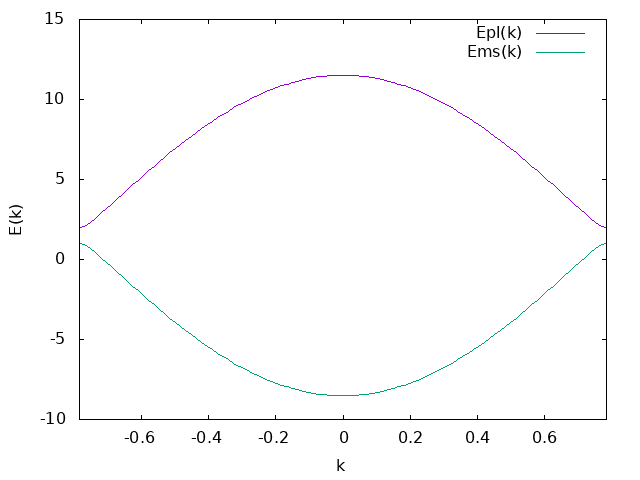
\includegraphics[scale=.8]{plot2.png}
\]
and in the extended zone scheme
\[
  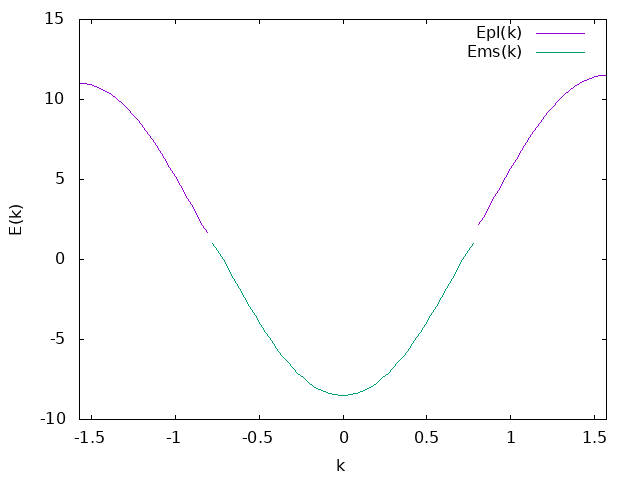
\includegraphics[scale=.8]{plot3.png}
\]
In the limit as $t\to 0$, $E\to \epsilon_{A}+\epsilon_{B}$ for the positive branch
and $E\to0$ for the negative branch.
Near the minimum, we can expand near $k=0$ $\cos(ka)\approx 1-k^{2}a^{2}/2$ to get
\[
  E\approx(\epsilon_{A}+\epsilon_{B})/2-\frac{1}{2}\sqrt{(\epsilon_{A}-\epsilon_{B})^{2}+4t^{2}[4-k^{2}a^{2}]}
\]
Expanding again using $\sqrt{a+x}\approx\sqrt{a}+\frac{x}{2\sqrt{a}}$,
\[
  E\approx (\epsilon_{A}+\epsilon_{B})/2-\frac{\sqrt{(\epsilon_{A}-\epsilon_{B})^{2}+16t^{2}}}{2}+\frac{1}{2}
  \frac{4t^{2}a^{2}k^{2}}{2\sqrt{(\epsilon_{A}-\epsilon_{B})^{2}+16t^{2}}}
  =\textrm{const}+\frac{t^{2}a^{2}k^{2}}{\sqrt{(\epsilon_{A}-\epsilon_{B})^{2}+16t^{2}}}
\]
Setting the quadratic part of this equation equal to the free electron dispersion,
\[
  \frac{\hbar^{2}k^{2}}{2m^{*}}=\frac{t^{2}a^{2}k^{2}}{\sqrt{(\epsilon_{A}-\epsilon_{B})^{2}+16t^{2}}}
  \Leftrightarrow m^{*}=\frac{\hbar^{2}\sqrt{(\epsilon_{A}-\epsilon_{B})^{2}+16t^{2}}}{2a^{2}t^{2}}
\]
If each atom is monovalent, there are two electrons per unit cell, filling the band and resulting in an insulator.
If $\epsilon_{A}=\epsilon_{B}$, we recover the previous problem's monatomic tight-binding chain solution, and the material becomes a metal.

\section*{2}
From the periodic boundary conditions, we have in any dimension
\[
  e^{ik(x+L)}=e^{ikx}\Leftrightarrow e^{ikL}=1 \Leftrightarrow kL=2\pi n\Leftrightarrow k=2\pi n/L
\]
i.e. each eigenstate corresponds to a volume $(2\pi/L)^{3}$ in $k$-space;
the first Brillouin zone ranges from $-\pi/a$ to $\pi/a$ in each direction and so has volume $(2\pi/a)^3$.
Dividing by the $k$-volume per eigenstate, there are $(L/a)^{3}$ eigenstates in the first Brillouin zone.
But this is exactly the expression for the number of primitive unit cells in the sample, which is the desired result.

\section*{3}
Since the potential is weak, the motion of the electrons is approximately free, and so a plane-wave state is a good approximation
to the solution.
Degenerate second-order perturbation theory implies that wave functions near the zone boundary may be decomposed
\[
  \Psi = A|k\rangle+B|k+G\rangle = Ae^{ikx}+Be^{i(k+G)x}
\]
We have an effective Schr\"odinger equation
\[
  \begin{pmatrix}
    \epsilon_{0}(k) & V_{G}^{*} \\
    V_{G} & \epsilon_{0}(k+G)
  \end{pmatrix}
  \begin{pmatrix}
    A \\
    B
  \end{pmatrix}
  =E
  \begin{pmatrix}
    A \\
    B
  \end{pmatrix}
\]
which is an eigenvalue problem equivalent to
\[
  0=
  \begin{vmatrix}
    \epsilon_{0}(k)-E & V_{G}^{*} \\
    V_{G} & \epsilon_{0}(k+G)-E
  \end{vmatrix}
  =\epsilon_{0}(k)\epsilon_{0}(k+G)-[\epsilon_{0}(k)+\epsilon_{0}(k+G)]E+E^{2}-|V_{G}|^{2}
\]
\[
  \Leftrightarrow E=\frac{\epsilon_{0}(k)+\epsilon_{0}(k+G)\pm
    \sqrt{[\epsilon_{0}(k)+\epsilon_{0}(k+G)]^{2}-4(\epsilon_{0}(k)\epsilon_{0}(k+G)-|V_{G}|^{2})}}{2}
\]
\[
  =\frac{1}{2}\left( \epsilon_{0}(k)+\epsilon_{0}(k+G)\pm
    \sqrt{[\epsilon_{0}(k)-\epsilon_{0}(k+G)]^{2}+4|V_{G}|^{2}} \right)
\]
Exactly on the Brillouin zone boundary, $\epsilon_{0}(k)=\epsilon_{0}(k+G)$, so
\[E=\epsilon\pm|V_{G}|\]
Applying the dispersion of the free electron,
\[
  E=\frac{\hbar^{2}k^{2}}{2m}+V_{0}\pm|V_{G}|
\]
The states are separated by $2|V_{G}|$ because the potential $V_{G}$ causes the scattered state to interfere with the incident state,
producing two states with different energies.
With a rather exaggerated band gap, the dispersion in the reduced zone scheme is sketched as
\[
  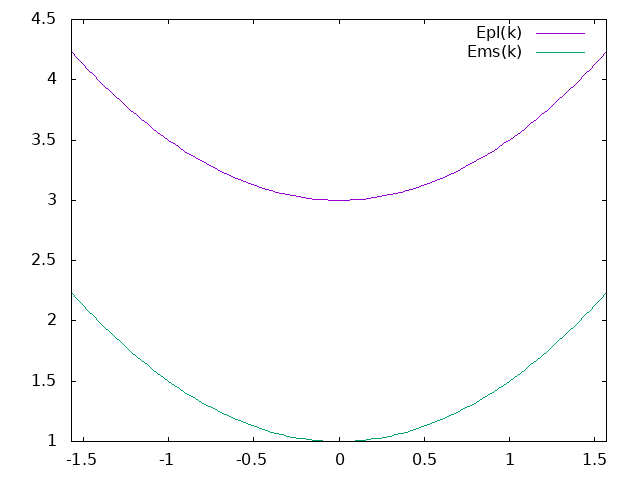
\includegraphics[scale=.8]{plot4.png}
\]
and in the extended zone scheme as
\[
  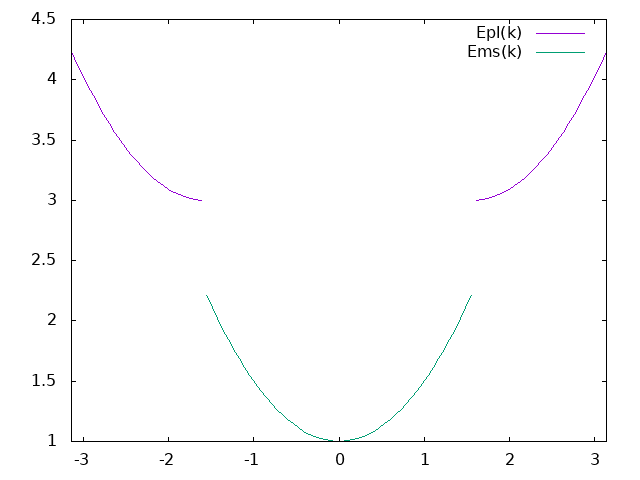
\includegraphics[scale=.8]{plot5.png}
\]
A plane wave near the Brillouin zone boundary with $k=n\pi/a+\delta$ can scatter off the periodic potential to $k'=-n\pi/a+\delta$
The energies corresponding to these waves are
\[
  \epsilon_{0}(n\pi/a+\delta)=\frac{\hbar^{2}}{2m}[(n\pi/a)^{2}+2n\pi\delta/a+\delta^{2}]
\]
\[
  \epsilon_{0}(-n\pi/a+\delta)=\frac{\hbar^{2}}{2m}[(n\pi/a)^{2}-2n\pi\delta/a+\delta^{2}]
\]
Using the characteristic equation derived from degenerate perturbation theory,
\[
  \left( \epsilon_{0}(\vec{k})-E \right)\left( \epsilon_{0}(\vec{k}+\vec{G})-E \right)-|V_{\vec{G}}|^{2}=0
\]
\[
  \Leftrightarrow\left(\frac{\hbar^{2}}{2m}[(n\pi/a)^{2}+2n\pi\delta/a+\delta^{2}] -E \right)
  \left( \frac{\hbar^{2}}{2m}[(n\pi/a)^{2}-2n\pi\delta/a+\delta^{2}]-E \right)-|V_{\vec{G}}|^{2}=0
\]
\[
  \Leftrightarrow E^{2}-E\frac{\hbar^{2}}{m}\left( (n\pi/a)^{2}+\delta^{2} \right)
  +\frac{\hbar^{4}}{4m^{2}}\left( (n\pi/a)^{2}-2n\pi\delta/a +\delta^{2}\right)\left( (n\pi/a)^{2}+2n\pi\delta/a+\delta^{2}\right)
  -|V_{G}|^{2}=0
\]
\[
  \Rightarrow E=\frac{ \frac{\hbar^{2}}{m}((n\pi/a)^{2}+\delta)}{2}
\]
\[
  \pm\frac{\sqrt{\frac{\hbar^{4}}{m^{2}}[(n\pi/a)^{2}+\delta^{2}]^{2}-\frac{\hbar^{4}}{m^{2}}\left( (n\pi/a)^{2}-2n\pi\delta/a
      +\delta^{2}\right)\left( (n\pi/a)^{2}+2n\pi\delta/a+\delta^{2}\right)}-4|V_{G}|^{2}}{2}
\]
\[
  \Leftrightarrow E=\frac{\hbar^{2}}{2m}[(n\pi/a)^{2}+\delta^{2}]
  \pm\sqrt{\left( \frac{\hbar^{2}}{2m}2n\pi\delta/a \right)^{2}+|V_{G}|^{2}}
\]
Expanding $\sqrt{a+x}\approx\sqrt{a}+\frac{x}{2\sqrt{a}}$,
\[
  E\approx \frac{\hbar^{2}}{2m}(n\pi/a)^{2}\pm|V_{G}|+\frac{\hbar^{2}\delta^{2}}{2m}\left[ 1\pm\frac{\hbar^{2}}{m}(n\pi/a)^{2}\frac{1}{|V_{G}|} \right]
\]
Under this approximation, the effective mass is, taking the dispersion relation above evaluated at $\delta=k$ and dropping the additive
constants,
\[
  \frac{\hbar^{2}k^{2}}{2m^{*}}=\frac{\hbar^{2}k^{2}}{2m}\left[ 1\pm\frac{\hbar^{2}}{m}(n\pi/a)^{2}\frac{1}{|V_{G}} \right]
\]
\[
  \Leftrightarrow m^{*}=\frac{m}{1\pm\frac{\hbar^{2}}{m}(n\pi/a)^{2}\frac{1}{|V_{G}|}}
\]
As the potential increases, the Fermi sea is pulled closer to the Brillouin zone boundary.
It is important to note we have divalent atoms, so the zone is actually filled.
In the case of a weak potential, the Fermi sea is approximately circular:
\begin{center}
  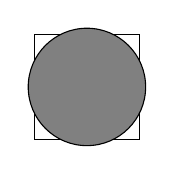
\begin{tikzpicture}[square/.style={regular polygon,regular polygon sides=4}]
    \node[scale=4] at (0,0) [square,draw] {};
    \node[scale=4.5] at (0,0) [circle,draw,fill=gray] {};
  \end{tikzpicture}
\end{center}
In the case of an intermediately strong potential, the Fermi sea gets pulled towards the zone boundary, but not so much that it fills the
zone with no gaps:
\begin{center}
  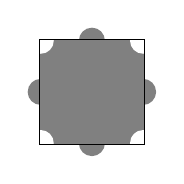
\begin{tikzpicture}[square/.style={regular polygon,regular polygon sides=4}]

    \node[scale=4] at (0,0) [square,fill=gray] {};

    \node at (.65,.65) [circle,fill=white] {};
    \node at (.65,-.65) [circle,fill=white] {};
    \node at (-.65,.65) [circle,fill=white] {};
    \node at (-.65,-.65) [circle,fill=white] {};

    \node at (0,-.65) [circle,fill=gray] {};
    \node at (-.65,0) [circle,fill=gray] {};
    \node at (.65,0) [circle,fill=gray] {};
    \node at (0,.65) [circle,fill=gray] {};

    \node[scale=4] at (0,0) [square,draw] {};
  \end{tikzpicture}
\end{center}
In the case of a very strong potential, the Fermi sea is pulled very strongly towards the zone boundary and fills it with no gaps:
\begin{center}
  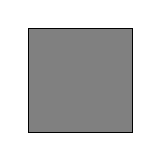
\begin{tikzpicture}[square/.style={regular polygon,regular polygon sides=4}]
    \node[scale=4] at (0,0) [square,draw,fill=gray] {};
  \end{tikzpicture}
\end{center}
The system is no longer a metal when there are no available states in the first Brillouin zone for traveling electrons to occupy.
This is characteristic only for strong potentials; exactly how strong this is may be estimated by noting the highest-energy
point in the first Brillouin zone is in the corner of the lattice with energy $\epsilon_{corner}=2\hbar^{2}\pi^{2}/2ma^{2}$,
and the lowest-energy state in the second zone is $\epsilon_{edga}=\hbar^{2}\pi^{2}/2ma^{2}$.
For the system to be an insulator, all the states in the first Brillouin zone must be lower in energy than any state in the second, so
that the zone is filled by the Fermi sea.
The rough condition for this to occur is $2\hbar^{2}\pi^{2}/2ma^{2}\leq \hbar^{2}\pi^{2}/2ma^{2}+V$, or
\[
  V\geq \frac{\hbar^{2}\pi^{2}}{4ma^{2}}
\]


\end{document}
%%% Local Variables:
%%% mode: latex
%%% TeX-master: t
%%% End:
